% ============================================================================
%  example_esco.tex  -- compact ESCO example for a single (double-column) column
%
%  Two high-specificity (leaf) IT occupations, their skills, one non-leaf skill
%  parent and one non-leaf occupation ancestor. All labels are REAL ESCO v1.2.1
%  concepts (domain: ICT / knowledge type):
%    Occupations : Systems analysts (ancestor) -> data analyst, data scientist
%    Skills      : database and network design and administration (parent) ->
%                  data models (shared), unstructured data, online analytical processing
%
%  Compile:  pdflatex example_esco.tex        (needs TikZ, no extra fonts)
% ============================================================================
\documentclass[border=3pt]{standalone}
\usepackage{tikz}
\usepackage[T1]{fontenc}
\renewcommand{\familydefault}{\sfdefault}
\usetikzlibrary{arrows.meta,positioning,backgrounds}

% --- palette taken from the pipeline figure --------------------------------
\definecolor{occLeaf}{HTML}{FCE3C1}   % warm peach  (occupation leaf)
\definecolor{occGrp} {HTML}{F4C98A}   % darker peach(occupation group)
\definecolor{skLeaf} {HTML}{CFE6F7}   % light blue  (skill leaf)
\definecolor{skGrp}  {HTML}{9FC9E8}   % darker blue (skill group)
\definecolor{shared} {HTML}{E8617A}   % coral       (shared relation)

\begin{document}
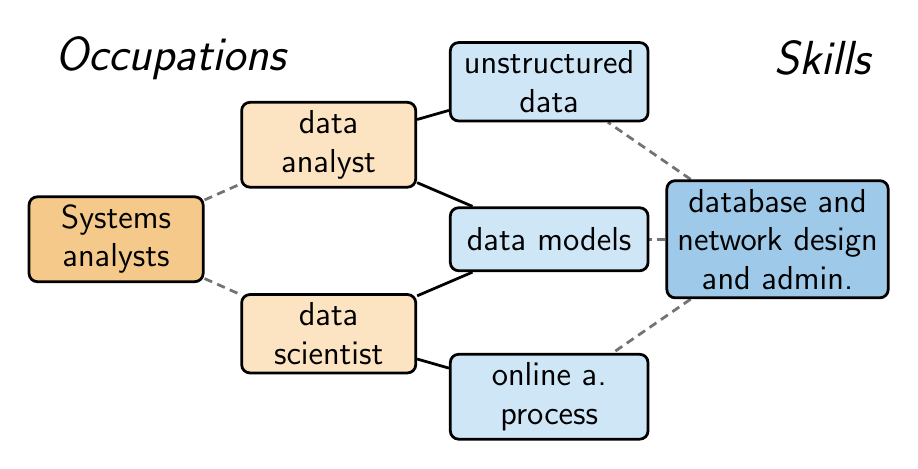
\begin{tikzpicture}[
  font=\large,
  >={Latex[length=2.4mm]},
  node/.style={draw=black,line width=1pt,rounded corners=3pt,align=center,
               text width=20mm,inner sep=3pt,minimum height=8mm},
  occL/.style={node,fill=occLeaf},
  occG/.style={node,fill=occGrp,line width=1pt},
  skL/.style={node,fill=skLeaf,text width=23mm},
  skG/.style={node,fill=skGrp,line width=1pt,text width=26mm},
  broader/.style={densely dashed,draw=black!55,line width=1pt},
  ess/.style={draw=black,line width=1pt},
  essShared/.style={draw=black,line width=1pt},
]

% ---- column headers -------------------------------------------------------
\node[anchor=west,font=\LARGE\itshape] at (-0.9,4.6) {Occupations};
\node[anchor=east,font=\LARGE\itshape] at ( 9.7,4.6) {Skills};

% ---- nodes (layered left -> right) ----------------------------------------
\node[occG] (sa)   at (0.0,2.3) {Systems analysts};
\node[occL] (da)   at (2.7,3.5) {data analyst};
\node[occL] (ds)   at (2.7,1.1) {data scientist};

\node[skL]  (ud)   at (5.5,4.3) {unstructured data};
\node[skL]  (dm)   at (5.5,2.3) {data models};
\node[skL]  (olap) at (5.5,0.3) {online a. process};

\node[skG]  (skg)  at (8.4,2.3) {database and network design and admin.};

% ---- edges on background layer so boxes stay readable ---------------------
\begin{scope}[on background layer]
  % occupation taxonomy (broader)
  \draw[broader] (sa) -- (da);
  \draw[broader] (sa) -- (ds);
  % skill taxonomy (broader)
  \draw[broader] (skg) -- (ud);
  \draw[broader] (skg) -- (dm);
  \draw[broader] (skg) -- (olap);
  % essential (occupation -> skill)
  \draw[ess]       (da) -- (ud);
  \draw[essShared] (da) -- (dm);   % shared
  \draw[essShared] (ds) -- (dm);   % shared
  \draw[ess]       (ds) -- (olap);
\end{scope}

\end{tikzpicture}
\end{document}
